\documentclass[12pt]{article}
\usepackage[left=0.9in, right=0.9in, top=1in, bottom=1in]{geometry}
\usepackage{tikz}
\usepackage{setspace}
\usepackage{hyperref}
\usepackage{amsfonts, amssymb, amsmath} 
\usepackage{titlesec}
\usepackage{pgfplots}
\pgfplotsset{compat=1.18}
\usepackage{graphicx}
\usepackage{wrapfig}
\usepackage{caption}
\usepackage{enumitem}
\usetikzlibrary{shadows.blur}
\usepackage{lmodern}
\setlength{\parskip}{0pt}
\setlength{\parindent}{0pt}

\title{\textcolor{purple}{\Huge\textbf{Analízis alkalmazásai}}}
\author{1. gyakorlat}
\date{Szabó Krisztián}

\renewcommand{\contentsname}{Tartalom}
\newcommand{\R}{\mathbb{R}}
\newcommand{\N}{\mathbb{N}}
\newcommand{\E}{\exists}
\newcommand{\mm}{\mathbf{m}}
\newcommand{\MM}{\mathbf{M}}
\newcommand{\K}{\mathbb{K}}
\newcommand{\D}{\mathcal{D}_f}

\definecolor{modernyellow}{HTML}{F4E4BC}
\definecolor{moderngreen}{HTML}{BDDCBD}

\tikzset
{
	definition/.style={
		draw,
		fill=modernyellow,
		line width=1pt,
		rounded corners,
		drop shadow={shadow blur steps=5,shadow xshift=1ex,shadow yshift=-1ex},
		text width=0.9\textwidth,
		inner sep=10pt
	},
	theorem/.style={
		draw,
		fill=moderngreen,
		line width=1pt,
		rounded corners,
		drop shadow={shadow blur steps=5,shadow xshift=1ex,shadow yshift=-1ex},
		text width=0.9\textwidth,
		inner sep=10pt
	},
	proof/.style={
		fill=white,
		rectangle,
		drop shadow={shadow blur steps=5,shadow xshift=1ex,shadow yshift=-1ex, moderngreen},
		text width=0.9\textwidth,
		inner sep=6pt,
	},
	proof1/.style={
		fill=white,
		rectangle,
		drop shadow={shadow blur steps=5,shadow xshift=1ex,shadow yshift=0, moderngreen},
		text width=0.9\textwidth,
		inner sep=6pt,
	}
}

\begin{document}
    \maketitle
    \tableofcontents
    \newpage
    \section{Emlékeztető}
    \subsection{Paraméteres integrál}
	Valamilyen kompakt $[a, \, b]$ intervallum $(a, \, b \in \R, \, a < b)$ és $\emptyset \neq U \subset \R^n$ $(1 \leq n \in \N)$ nyílt halmaz esetén tekintsük az
	\[
		f : U \times [a, \, b] \to \R
	\]
	függvényt. Ha $x \in U$, akkor legyen $f_x : [a, \, b] \to \R$ az a függvény, amire
	\[
		f_x(t) := f(x, \, t) \quad (t\in [a, \, b]).
	\]
	Tegyük fel, hogy minden $x \in U$ esetén az $f_x$ függvény Riemann-integrálható: $f_x \in R[a, \, b]$, legyen ekkor
	\[
		F(x) := \int\limits_a^b f(x, \, t) \, dt := \int\limits_a^b f_x \quad (x \in U).
	\]

	\tikz \node[theorem]
	{
		\textbf{Tétel.} Tegyük fel, hogy adott az $[a, \, b]$ $(a, \, b \in \R, \, a < b)$ kompakt intervallum, $1 \leq n \in \N$, és $\emptyset \neq U \subset \R^n$ nyílt halmaz. Ekkor tetszőleges folytonos
		\[
			f : U \times [a, \, b] \to \R
		\]
		függvény esetén az
		\[
			F(x) := \int\limits_a^b f(x, \, t) \, dt \quad (x \in U)
		\]
		paraméteres integrálra az alábbiak igazak:
		\begin{enumerate}
			\item az $F$ függvény folytonos;
			\item ha valamilyen $i = 1, \, \dots, \, n$ indexre létezik és folytonos a $\partial_i f$ parciális deriváltfüggvény, akkor létezik a $\partial_i F$ parciális deriváltfüggvény is, és
			\[
				\partial_i F(x) = \int\limits_a^b \partial_i f(x, \, t) \, dt \quad (x \in U);
			\]
			\item amennyiben az $f$ folytonosan differenciálható, azaz $f \in C^1$, akkor $F \in C^1$.
		\end{enumerate}
	};\newline
	
	\tikz \node[proof1]
	{
		\textbf{Bizonyítás.} Az $F$ függvény valamely $x \in U$ pontbeli folytonosságához az
		\[
			F(x) - F(y) = \int\limits_a^b \big( f(x, \, t)  - f(y, \, t) \big) \quad (y \in U)
		\]
		különbséget, azaz az
		\[
			f(x, \, t) - f(y, \, t) \quad (t \in [a, \, b])
		\]
	};

	\tikz \node[proof]
	{
		megváltozoást kell "kezelni". Legyen ehhez tehát adotot az $x \in U$ vektor, ekkor az $U$ halmaz nyíltsága miatt egy alkalmas $r > 0$ számmal
		\[
			G_r := \{ y \in U : ||x - y|| \leq r \} \subset U.
		\]
		A $G_r$ halmaz könnyen láthatóan zárt, ezért az
		\[
			A := G_r \times [a, \, b] \, (\subset U \times [a, \, b] = \D)
		\]
		halmaz is zárt. Mivel az $A$ nyilván korlátos is, így kompakt. A Heine-tétel alapján az $f_{|A}$ leszűkítés egyenletesen folytonos, tehát tetszőleges $\varepsilon > 0$ számhoz van olyan $\delta > 0$, hogy
		\[
			|f(\xi) - f(\zeta)| < \varepsilon \quad (\xi, \, \zeta \in A, \, ||\xi - \zeta|| < \delta).
		\]
	};\newline
	
	%%% Implicitfüggvény-tétel margó
	%%% Inverzfüggvény-tétel margó
	%%% Differenciálegyenletek

	\begin{center}
		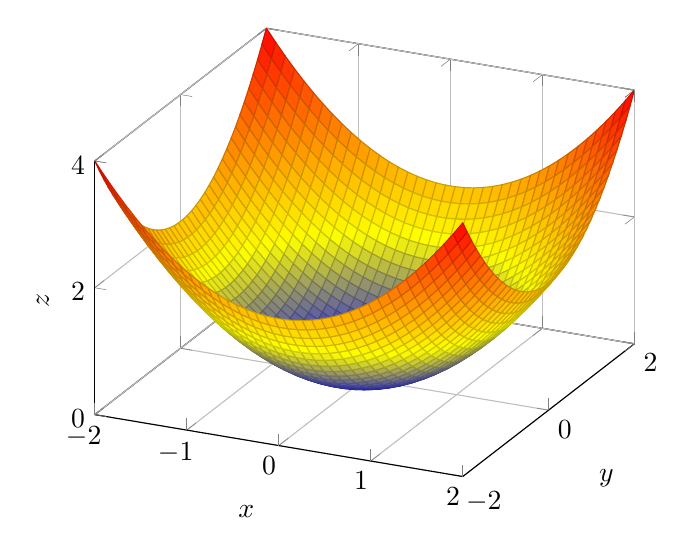
\begin{tikzpicture}
			\begin{axis}[
			  xlabel={$x$},
			  ylabel={$y$},
			  zlabel={$z$},
			  grid=major,
			  zmin=0,
			  zmax=4,
			  domain=-2:2,
			]
			  \addplot3[surf, domain=-2:2, samples=40] {(x^2 + y^2) / 2}; 
			\end{axis}
		  \end{tikzpicture}
	\end{center}
	

\end{document}